% Drawing 86/01-7 -- folder 86, batch 01, archive page 7 (PDF page 8).
% Transcription: en haut, (B$_1$) : l'icosaèdre en perspective, vu le long d'un axe passant par les centres de deux faces opposées, arêtes cachées en tirets ; sommets du contour $u_1$ (en haut), $v'_1$, $w_1$, $u'_1$ (en bas), $v_1$, $w'_1$ ; face avant $w$, $v$, $u$ ; face arrière $u'$, $v'$, $w'$.
% Kind: icosahedron in perspective along a 3-fold axis, named vertices. Method 2 (schematic redraw from the facsimile). Status: ok.
% Notes: Drawn from the twelve vertices as read and the edges of the page: the hexagonal outline u_1, v'_1, w_1, u'_1, v_1, w'_1; the front face w, v, u and its nine edges to the outline, solid; the back face u', v', w' and its nine edges to the outline, dashed (30 edges). Labels as on the page (outer ones outside the outline, inner ones beside their vertices). Stroke weights are not reproduced. The transcription's note lists some of the names with a question mark (« w'_1 (?) »): the upper left vertex is read w'_1 here, the upper right v'_1, which fits the rule of the page (T, T_1, T'_1, T' with opposite vertices x and x'). Redrawn 2026-11-12 (issue 128): to check again.
% Coordinates: 1 unit = 1 mm = 1/100 of the crop width (bbox in page fractions: [0.22, 0.09, 0.56, 0.37]).
% Redrawn by Claude (claude-fable-5-2), issue #128, 2026-11-12; not checked by a human; not compiled (no TeX in the session).
% Rights: reproduces part of the work -- behind RENDER_TRANSCRIPTS, never published by itself.
\documentclass[tikz,border=3pt]{standalone}
\usepackage{amsmath,amssymb}
\usetikzlibrary{patterns,arrows.meta}
\tikzset{pencil/.style={black!45}, struck/.style={black!35}, mpt/.style={circle,draw,inner sep=1.3pt}, pt/.style={circle,fill,inner sep=0.9pt}, opt/.style={circle,draw,fill=white,inner sep=1.1pt}}
\begin{document}
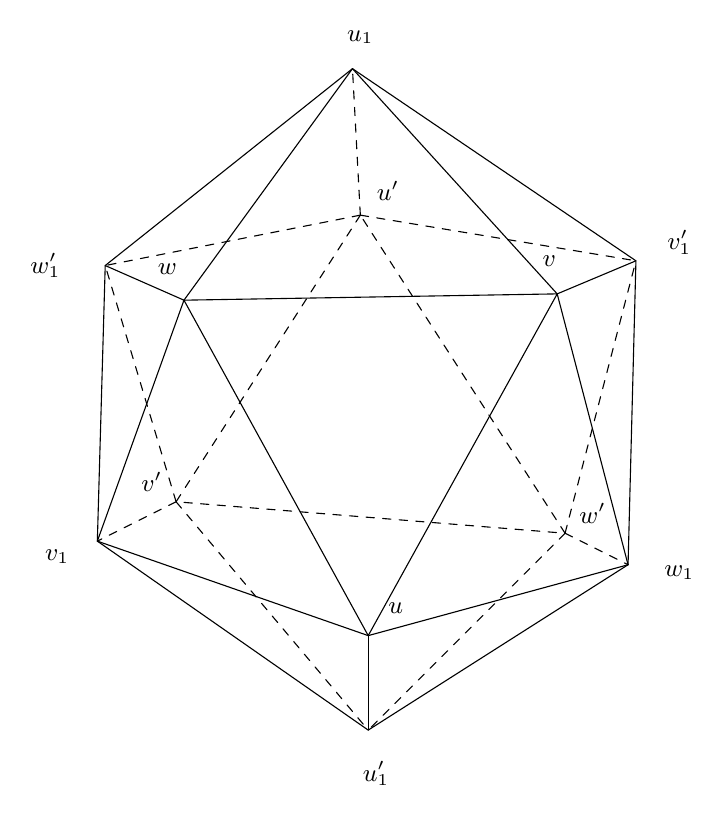
\begin{tikzpicture}[x=1mm,y=1mm,line cap=round,line join=round,font=\scriptsize]
\draw (52,-16) -- (88,-40.4) -- (87,-79) -- (54,-100) -- (19.6,-76) -- (20.6,-41) -- cycle;
\draw (30.6,-45.4) -- (78,-44.6) -- (54,-88) -- cycle;
\draw (30.6,-45.4) -- (20.6,-41);
\draw (30.6,-45.4) -- (52,-16);
\draw (30.6,-45.4) -- (19.6,-76);
\draw (78,-44.6) -- (52,-16);
\draw (78,-44.6) -- (88,-40.4);
\draw (78,-44.6) -- (87,-79);
\draw (54,-88) -- (19.6,-76);
\draw (54,-88) -- (54,-100);
\draw (54,-88) -- (87,-79);
\draw[dashed] (53,-34.6) -- (29.6,-71) -- (79,-75) -- cycle;
\draw[dashed] (53,-34.6) -- (52,-16);
\draw[dashed] (53,-34.6) -- (20.6,-41);
\draw[dashed] (53,-34.6) -- (88,-40.4);
\draw[dashed] (29.6,-71) -- (20.6,-41);
\draw[dashed] (29.6,-71) -- (19.6,-76);
\draw[dashed] (29.6,-71) -- (54,-100);
\draw[dashed] (79,-75) -- (88,-40.4);
\draw[dashed] (79,-75) -- (87,-79);
\draw[dashed] (79,-75) -- (54,-100);
\node[inner sep=1pt] at (53,-12) {\small $u_1$};
\node[inner sep=1pt] at (93.5,-38) {\small $v'_1$};
\node[inner sep=1pt] at (93.5,-80) {\small $w_1$};
\node[inner sep=1pt] at (55,-105.5) {\small $u'_1$};
\node[inner sep=1pt] at (14.5,-78) {\small $v_1$};
\node[inner sep=1pt] at (13,-41) {\small $w'_1$};
\node[inner sep=1pt] at (28.5,-41.5) {\small $w$};
\node[inner sep=1pt] at (77,-40.5) {\small $v$};
\node[inner sep=1pt] at (57.5,-84.5) {\small $u$};
\node[inner sep=1pt] at (56.5,-31.5) {\small $u'$};
\node[inner sep=1pt] at (26.5,-68.5) {\small $v'$};
\node[inner sep=1pt] at (82.5,-72.5) {\small $w'$};
\end{tikzpicture}
\end{document}
